% stumps.tex
% Jeremy Barnes, 22/9/1999
% $Id$

\chapter{Decision Stumps}
\label{chapter:stumps}

We digress slightly from the theory to look at a simple example of a
practical learning machine, that has some nice properties (and was used
to perform all of the experiments in this thesis).
The \emph{decision stumps} algorithm is a very simple learning
machine.  As a standalone tool it is almost useless; but when
combined with the boosting algorithm it can generate very good
hypotheses.  Additionally, it has a fixed VC dimension which aids in
the analysis of learning algorithms based upon it.

\section{The decision stump learning machine}

The decision stump algorithm divides the input space into two disjoint
regions, with the boundary between them running perpendicular to one
of the axes (the decision boundary is an axis-orthogonal hyperplane).
Each region is given a label.  Figure \ref{fig:decision stump} shows
the decision boundaries of two decision stump classifiers.

\begin{linefigure}
\begin{center}
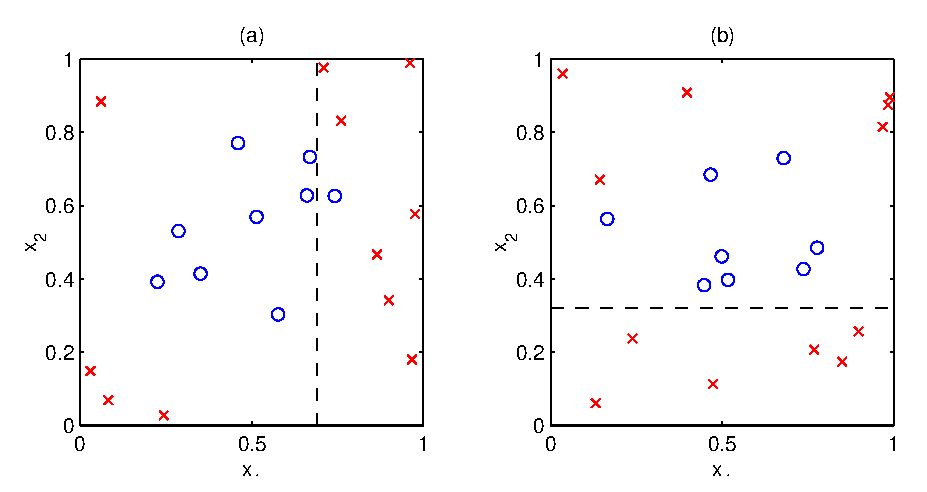
\includegraphics{figures/stumpdiagram.epsg}
\end{center}
\begin{capt}{A decision stump classifier}{fig:decision stump}
Part (a) shows the decision boundary of a decision stump classifier,
and the label of each region.  Part (b) the data it was trained on,
where $\times = -1$ and $\circ = +1$.
\end{capt}
\end{linefigure}

The algorithm constructs a list of possible split locations and
exhaustively searches this list for the minimum of the cost function
(misclassification risk).  Possible split locations are determined by
projecting every data point onto each axis in turn, and bisecting each
pair of consecutive projections to determine the candidate point.
Figure \ref{fig:candidate points} illustrates the process.

\begin{linefigure}
\begin{center}
\includegraphics{figures/stumpcandidates.epsg}
\end{center}
\begin{capt}{Candidate points for decision stump split}{fig:candidate points}
Data points ($\times$) are projected onto the axes.  Each consecutive
pair of projections is then bisected, to generate candidate split
points ($\bullet$).
\end{capt}
\end{linefigure}

\section{Properties of decision stumps}

\begin{theorem}[VC dimension of decision stumps]
\label{theorem:vcdim stumps}
The set $\mathcal{S}$ of decision stump classifiers on an domain
$\calI \subseteq \bbR^d$ has a VC dimension of bounded by 
%
\begin{equation}
\VCdim(\calS) \leq d + 1
\end{equation}
%
and, for a training set $X$ of size $m \gg d$ with sufficient
variation in its $\bfx$ parameters, has a constant VC dimension.
%
\end{theorem}

\proof The set $\calS$ of all axis orthogonal hyperplanes
is contained within the set $\calH$ of $d$ dimensional hyperplanes
(which has VC dimension $d+1$.

That the VC dimension is constant is intuitively sensible
but tricky to prove formally.  As no subsequent result \emph{relies}
upon this property, we will not elaborate further.




